\chapter{Primeira fase de implementa��o}
\section{Placa PCI do primeiro prot�tipo}
\begin{figure}[H]
	\centering
	\begin{subfigure}{.48\textwidth}
		\centering
		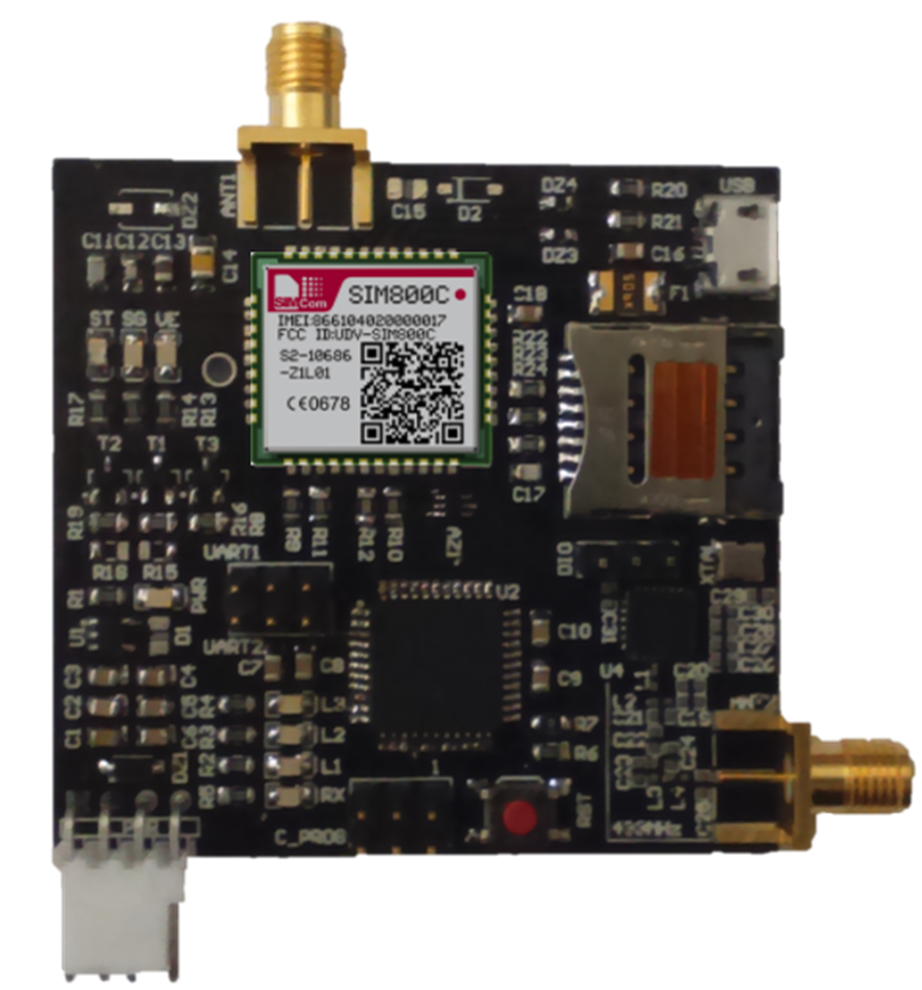
\includegraphics[width=0.8\linewidth]{Figuras/prototop}
		\captionsetup{labelformat=empty}
		\caption{(a) Top layer.}
	\end{subfigure}%
	\hspace{0.1cm}
	\begin{subfigure}{.48\textwidth}
		\centering
		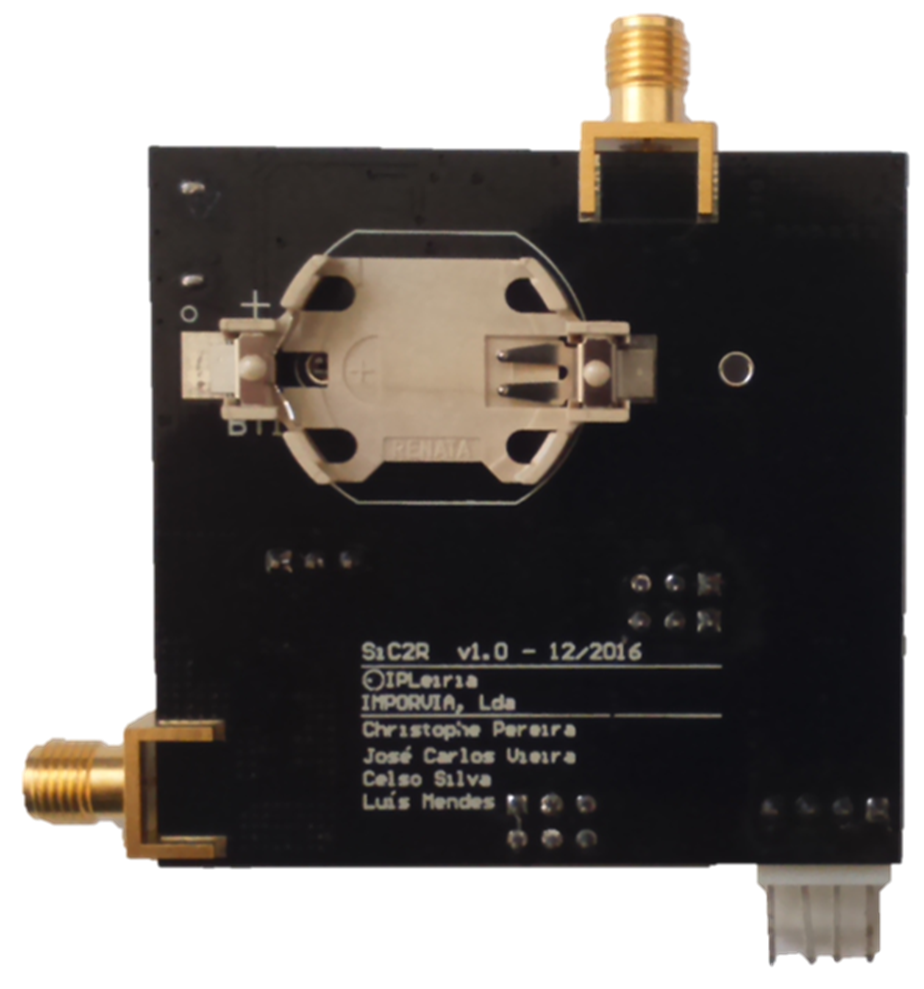
\includegraphics[width=0.8\linewidth]{Figuras/protobott}
		\captionsetup{labelformat=empty}
		\caption{(b) Botton layer.}
	\end{subfigure}
	\caption{PCI do primeiro prot�tipo.}
\end{figure}
\section{Placa de comandos}
\begin{figure}[H]
	\centering
	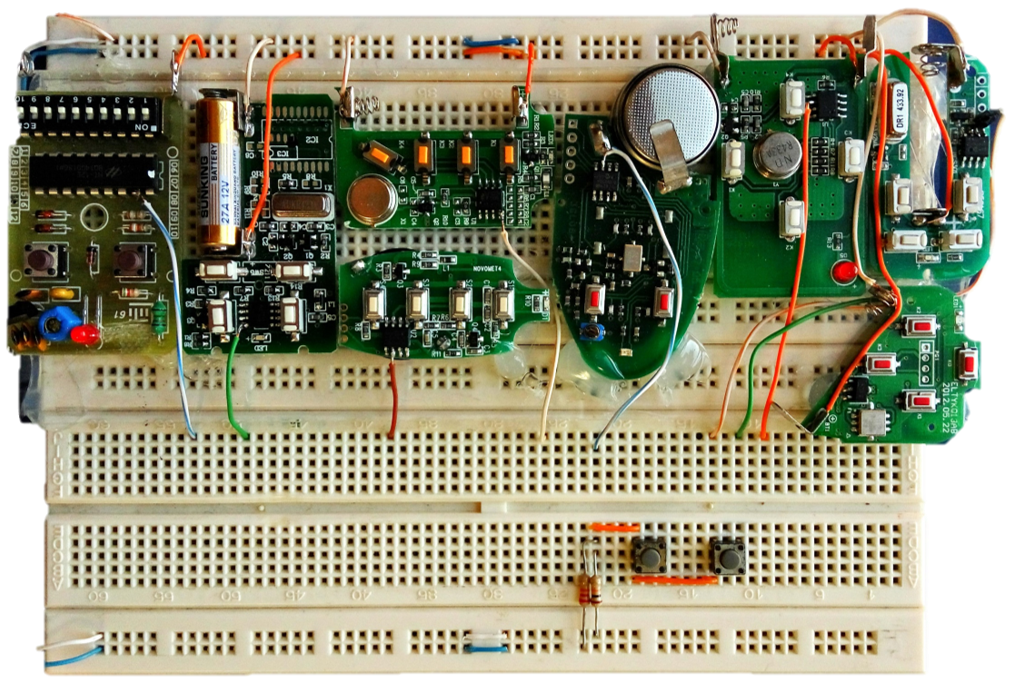
\includegraphics[width=0.6\linewidth]{Figuras/placa_comandos}
	\caption{Placa de comandos utilizados para teste.}
\end{figure}\vfill\pagebreak\thispagestyle{plain}

\chapter{\textit{Pinout} do microcontrolador}
\begin{figure}[H]
	\centering
	\includegraphics[clip, trim=3cm 2.1cm 3cm 1.91cm, width=0.64\linewidth]{Figuras/Anexos/pinout}
	\caption{Tabela de correspond�ncia dos pinos do microcontrolador.}
	\label{fig:pinout}
\end{figure}\vfill\pagebreak\thispagestyle{plain}

\chapter{Antenas}\label{antenasanexo}
\section{Antena de desenvolvimento}
\begin{figure}[H]
	\centering
	\tabskip=0pt
	\hbox{
		\begin{subfigure}{\textwidth}
			\centering
			\includegraphics[clip, trim=1.5cm 6.8cm 1.5cm 8.5cm, width=0.8\linewidth]{Antenas/Antena433MHz/Antena433Mhz}
			\captionsetup{labelformat=empty}
			\caption{(a) Par�metro S11.}
		\end{subfigure}
	}
	\vspace{0.5cm}
	\hbox{
		\begin{subfigure}{\textwidth}
			\centering
			\includegraphics[width=0.4\linewidth]{Antenas/Antena433MHz/Antena433MHz_fig}
			\captionsetup{labelformat=empty}
			\caption{(b) Antena.}
		\end{subfigure}
	}
	\caption{Antena de 433 MHz existente no mercado.}
\end{figure}
\section{Antena monopolo com meandro (0).}
\begin{figure}[H]
	\centering
	\tabskip=0pt
	\valign{#\cr
		\hbox{%
			\begin{subfigure}[b]{.3\textwidth}
				\centering
				\includegraphics[width=\textwidth]{Antenas/Set0/set0top}
				\caption{Top layer.}
			\end{subfigure}%
		}\vfill
		\hbox{%
			\begin{subfigure}[b]{.3\textwidth}
				\centering
				\includegraphics[width=\textwidth]{Antenas/Set0/set0bott}
				\caption{Bottom layer.}
			\end{subfigure}%
		}\cr
		\noalign{\hfill}
		\hbox{%
			\begin{subfigure}{.7\textwidth}
				\centering
				\includegraphics[clip, trim=1.5cm 6.8cm 1.5cm 8.5cm, width=0.9\linewidth]{Antenas/Set0/Set0}
				\caption{Par�metro S11.}
			\end{subfigure}%
		}\cr
	}
	\caption{Antena monopolo com meandro (0).}
\end{figure}
\section{Antena monopolo com meandro (1).}
\begin{figure}[H]
	\centering
	\tabskip=0pt
	\valign{#\cr
		\hbox{%
			\begin{subfigure}[b]{.3\textwidth}
				\centering
				\includegraphics[width=\textwidth]{Antenas/Set1/set1top}
				\caption{Top layer.}
			\end{subfigure}%
		}\vfill
		\hbox{%
			\begin{subfigure}[b]{.3\textwidth}
				\centering
				\includegraphics[width=\textwidth]{Antenas/Set1/set1bott}
				\caption{Bottom layer.}
			\end{subfigure}%
		}\cr
		\noalign{\hfill}
		\hbox{%
			\begin{subfigure}{.7\textwidth}
				\centering
				\includegraphics[clip, trim=1.5cm 6.8cm 1.5cm 8.5cm, width=0.9\linewidth]{Antenas/Set1/Set1}
				\caption{Par�metro S11.}
			\end{subfigure}%
		}\cr
	}
	\caption{Antena monopolo com meandro (1).}
\end{figure}
\section{Antena PIFA(Planar Inverted F Antenna) com um paralelo meandro (2)}
\begin{figure}[H]
	\centering
	\tabskip=0pt
	\valign{#\cr
		\hbox{%
			\begin{subfigure}[b]{.3\textwidth}
				\centering
				\includegraphics[width=\textwidth]{Antenas/Set2/set2top}
				\caption{Top layer.}
			\end{subfigure}%
		}\vfill
		\hbox{%
			\begin{subfigure}[b]{.3\textwidth}
				\centering
				\includegraphics[width=\textwidth]{Antenas/Set2/set2bott}
				\caption{Bottom layer.}
			\end{subfigure}%
		}\cr
		\noalign{\hfill}
		\hbox{%
			\begin{subfigure}{.7\textwidth}
				\centering
				\includegraphics[clip, trim=1.5cm 6.8cm 1.5cm 8.5cm, width=0.9\linewidth]{Antenas/Set2/Set2}
				\caption{Par�metro S11.}
			\end{subfigure}%
		}\cr
	}
	\caption{Antena PIFA(Planar Inverted F Antenna) com um paralelo meandro (2).}
\end{figure}
\section{Antena PIFA com meandro (3)}
\begin{figure}[H]
	\centering
	\tabskip=0pt
	\valign{#\cr
		\hbox{%
			\begin{subfigure}[b]{.3\textwidth}
				\centering
				\includegraphics[width=\textwidth]{Antenas/Set3/set3top}
				\caption{Top layer.}
			\end{subfigure}%
		}\vfill
		\hbox{%
			\begin{subfigure}[b]{.3\textwidth}
				\centering
				\includegraphics[width=\textwidth]{Antenas/Set3/set3bott}
				\caption{Bottom layer.}
			\end{subfigure}%
		}\cr
		\noalign{\hfill}
		\hbox{%
			\begin{subfigure}{.7\textwidth}
				\centering
				\includegraphics[clip, trim=1.5cm 6.8cm 1.5cm 8.5cm, width=0.9\linewidth]{Antenas/Set3/Set3}
				\caption{Par�metro S11.}
			\end{subfigure}%
		}\cr
	}
	\caption{Antena PIFA com meandro (3).}
\end{figure}
\section{Antena planar com meandro (4)}
\begin{figure}[H]
	\centering
	\tabskip=0pt
	\valign{#\cr
		\hbox{%
			\begin{subfigure}[b]{.3\textwidth}
				\centering
				\includegraphics[width=\textwidth]{Antenas/Set4/set4top}
				\caption{Top layer.}
			\end{subfigure}%
		}\vfill
		\hbox{%
			\begin{subfigure}[b]{.3\textwidth}
				\centering
				\includegraphics[width=\textwidth]{Antenas/Set4/set4bott}
				\caption{Bottom layer.}
			\end{subfigure}%
		}\cr
		\noalign{\hfill}
		\hbox{%
			\begin{subfigure}{.7\textwidth}
				\centering
				\includegraphics[clip, trim=1.5cm 6.8cm 1.5cm 8.5cm, width=0.9\linewidth]{Antenas/Set4/Set4}
				\caption{Par�metro S11.}
			\end{subfigure}%
		}\cr
	}
	\caption{Antena planar com meandro (4).}
\end{figure}
\section{Antena monopolo (5)}
\begin{figure}[H]
	\centering
	\tabskip=0pt
	\valign{#\cr
		\vspace{1.4cm}
		\hbox{%
			\begin{subfigure}[b]{.3\textwidth}
				\centering
				\includegraphics[width=\textwidth]{Antenas/Set5/set5top}
				\caption{Top layer.}
			\end{subfigure}%
		}\vspace{0.5cm}
		\hbox{%
			\begin{subfigure}[b]{.3\textwidth}
				\centering
				\includegraphics[width=\textwidth]{Antenas/Set5/set5bott}
				\caption{Bottom layer.}
			\end{subfigure}%
		}\cr
		\noalign{\hfill}
		\hbox{%
			\begin{subfigure}{.7\textwidth}
				\centering
				\includegraphics[clip, trim=1.5cm 6.8cm 1.5cm 8.5cm, width=0.9\linewidth]{Antenas/Set5/Set5}
				\caption{Par�metro S11.}
			\end{subfigure}%
		}\cr
	}
	\caption{Antena monopolo (5).}
\end{figure}
\section{Antena monopolo planar (6)}
\begin{figure}[H]
	\centering
	\tabskip=0pt
	\valign{#\cr
		\hbox{%
			\begin{subfigure}[b]{.3\textwidth}
				\centering
				\includegraphics[width=\textwidth]{Antenas/Set6/set6top}
				\caption{Top layer.}
			\end{subfigure}%
		}\vfill
		\hbox{%
			\begin{subfigure}[b]{.3\textwidth}
				\centering
				\includegraphics[width=\textwidth]{Antenas/Set6/set6bott}
				\caption{Bottom layer.}
			\end{subfigure}%
		}\cr
		\noalign{\hfill}
		\hbox{%
			\begin{subfigure}{.7\textwidth}
				\centering
				\includegraphics[clip, trim=1.5cm 6.8cm 1.5cm 8.5cm, width=0.9\linewidth]{Antenas/Set6/Set6}
				\caption{Par�metro S11.}
			\end{subfigure}%
		}\cr
	}
	\caption{Antena monopolo planar (6).}
\end{figure}
\section{Antena PIFA com meandro (7)}
\begin{figure}[H]
	\centering
	\tabskip=0pt
	\valign{#\cr
		\hbox{%
			\begin{subfigure}[b]{.3\textwidth}
				\centering
				\includegraphics[width=\textwidth]{Antenas/Set7/set7top}
				\caption{Top layer.}
			\end{subfigure}%
		}\vfill
		\hbox{%
			\begin{subfigure}[b]{.3\textwidth}
				\centering
				\includegraphics[width=\textwidth]{Antenas/Set7/set7bott}
				\caption{Bottom layer.}
			\end{subfigure}%
		}\cr
		\noalign{\hfill}
		\hbox{%
			\begin{subfigure}{.7\textwidth}
				\centering
				\includegraphics[clip, trim=1.5cm 6.8cm 1.5cm 8.5cm, width=0.9\linewidth]{Antenas/Set7/Set7}
				\caption{Par�metro S11.}
			\end{subfigure}%
		}\cr
	}
	\caption{Antena PIFA com meandro (7).}
\end{figure}
\section{Antena de teste 8}
\begin{figure}[H]
	\centering
	\tabskip=0pt
	\valign{#\cr
		\hbox{%
			\begin{subfigure}[b]{.3\textwidth}
				\centering
				\includegraphics[width=\textwidth]{Antenas/Set8/set8top}
				\caption{Top layer.}
			\end{subfigure}%
		}\vfill
		\hbox{%
			\begin{subfigure}[b]{.3\textwidth}
				\centering
				\includegraphics[width=\textwidth]{Antenas/Set8/set8bott}
				\caption{Bottom layer.}
			\end{subfigure}%
		}\cr
		\noalign{\hfill}
		\hbox{%
			\begin{subfigure}{.7\textwidth}
				\centering
				\includegraphics[clip, trim=1.5cm 6.8cm 1.5cm 8.5cm, width=0.9\linewidth]{Antenas/Set8/Set8}
				\caption{Par�metro S11.}
			\end{subfigure}%
		}\cr
	}
	\caption{Antena de teste 8.}
\end{figure}
\section{Antena monopolo com meandro (9)}
\begin{figure}[H]
	\centering
	\tabskip=0pt
	\valign{#\cr
		\hbox{%
			\begin{subfigure}[b]{.3\textwidth}
				\centering
				\includegraphics[width=\textwidth]{Antenas/Set9/set9top}
				\caption{Top layer.}
			\end{subfigure}%
		}\vfill
		\hbox{%
			\begin{subfigure}[b]{.3\textwidth}
				\centering
				\includegraphics[width=\textwidth]{Antenas/Set9/set9bott}
				\caption{Bottom layer.}
			\end{subfigure}%
		}\cr
		\noalign{\hfill}
		\hbox{%
			\begin{subfigure}{.7\textwidth}
				\centering
				\includegraphics[clip, trim=1.5cm 6.8cm 1.5cm 8.5cm, width=0.9\linewidth]{Antenas/Set9/Set9}
				\caption{Par�metro S11.}
			\end{subfigure}%
		}\cr
	}
	\caption{Antena monopolo com meandro (9).}
\end{figure}
\section{Antena monopolo com meandro (10)}
\begin{figure}[H]
	\centering
	\tabskip=0pt
	\valign{#\cr
		\hbox{%
			\begin{subfigure}[b]{.3\textwidth}
				\centering
				\includegraphics[width=\textwidth]{Antenas/Set10/set10top}
				\caption{Top layer.}
			\end{subfigure}%
		}\vfill
		\hbox{%
			\begin{subfigure}[b]{.3\textwidth}
				\centering
				\includegraphics[width=\textwidth]{Antenas/Set10/set10bott}
				\caption{Bottom layer.}
			\end{subfigure}%
		}\cr
		\noalign{\hfill}
		\hbox{%
			\begin{subfigure}{.7\textwidth}
				\centering
				\includegraphics[clip, trim=1.5cm 6.8cm 1.5cm 8.5cm, width=0.9\linewidth]{Antenas/Set10/Set10}
				\caption{Par�metro S11.}
			\end{subfigure}%
		}\cr
	}
	\caption{Antena monopolo com meandro (10).}
\end{figure}
\section{Antena monopolo com meandro (11)}
\begin{figure}[H]
	\centering
	\tabskip=0pt
	\valign{#\cr
		\hbox{%
			\begin{subfigure}[b]{.3\textwidth}
				\centering
				\includegraphics[width=\textwidth]{Antenas/Set11/set11top}
				\caption{Top layer.}
			\end{subfigure}%
		}\vfill
		\hbox{%
			\begin{subfigure}[b]{.3\textwidth}
				\centering
				\includegraphics[width=\textwidth]{Antenas/Set11/set11bott}
				\caption{Bottom layer.}
			\end{subfigure}%
		}\cr
		\noalign{\hfill}
		\hbox{%
			\begin{subfigure}{.7\textwidth}
				\centering
				\includegraphics[clip, trim=1.5cm 6.8cm 1.5cm 8.5cm, width=0.9\linewidth]{Antenas/Set11/Set11}
				\caption{Par�metro S11.}
			\end{subfigure}%
		}\cr
	}
	\caption{Antena monopolo com meandro (11).}
\end{figure}
\section{Antena monopolo com meandro (12)}
\begin{figure}[H]
	\centering
	\tabskip=0pt
	\valign{#\cr
		\hbox{%
			\begin{subfigure}[b]{.3\textwidth}
				\centering
				\includegraphics[width=\textwidth]{Antenas/Set12/set12top}
				\caption{Top layer.}
			\end{subfigure}%
		}\vfill
		\hbox{%
			\begin{subfigure}[b]{.3\textwidth}
				\centering
				\includegraphics[width=\textwidth]{Antenas/Set12/set12bott}
				\caption{Bottom layer.}
			\end{subfigure}%
		}\cr
		\noalign{\hfill}
		\hbox{%
			\begin{subfigure}{.7\textwidth}
				\centering
				\includegraphics[clip, trim=1.5cm 6.8cm 1.5cm 8.5cm, width=0.9\linewidth]{Antenas/Set12/Set12}
				\caption{Par�metro S11.}
			\end{subfigure}%
		}\cr
	}
	\caption{Antena monopolo com meandro (12).}
\end{figure}
\section{Antena monopolo com meandro (13)}
\begin{figure}[H]
	\centering
	\tabskip=0pt
	\valign{#\cr
		\hbox{%
			\begin{subfigure}[b]{.3\textwidth}
				\centering
				\includegraphics[width=\textwidth]{Antenas/Set13/set13top}
				\caption{Top layer.}
			\end{subfigure}%
		}\vfill
		\hbox{%
			\begin{subfigure}[b]{.3\textwidth}
				\centering
				\includegraphics[width=\textwidth]{Antenas/Set13/set13bott}
				\caption{Bottom layer.}
			\end{subfigure}%
		}\cr
		\noalign{\hfill}
		\hbox{%
			\begin{subfigure}{.7\textwidth}
				\centering
				\includegraphics[clip, trim=1.5cm 6.8cm 1.5cm 8.5cm, width=0.9\linewidth]{Antenas/Set13/Set13}
				\caption{Par�metro S11.}
			\end{subfigure}%
		}\cr
	}
	\caption{Antena monopolo com meandro (13).}
\end{figure}
\section{Antena monopolo com meandro (14)}
\begin{figure}[H]
	\centering
	\tabskip=0pt
	\valign{#\cr
		\hbox{%
			\begin{subfigure}[b]{.3\textwidth}
				\centering
				\includegraphics[width=\textwidth]{Antenas/Set14/set14top}
				\caption{Top layer.}
			\end{subfigure}%
		}\vfill
		\hbox{%
			\begin{subfigure}[b]{.3\textwidth}
				\centering
				\includegraphics[width=\textwidth]{Antenas/Set14/set14bott}
				\caption{Bottom layer.}
			\end{subfigure}%
		}\cr
		\noalign{\hfill}
		\hbox{%
			\begin{subfigure}{.7\textwidth}
				\centering
				\includegraphics[clip, trim=1.5cm 6.8cm 1.5cm 8.5cm, width=0.9\linewidth]{Antenas/Set14/Set14}
				\caption{Par�metro S11.}
			\end{subfigure}%
		}\cr
	}
	\caption{Antena monopolo com meandro (14).}
\end{figure}
\section{Antena monopolo de duas camadas em espiral (15)}
\begin{figure}[H]
	\centering
	\tabskip=0pt
	\valign{#\cr
		\hbox{%
			\begin{subfigure}[b]{.3\textwidth}
				\centering
				\includegraphics[width=\textwidth]{Antenas/Set15/set15top}
				\caption{Top layer.}
			\end{subfigure}%
		}\vfill
		\hbox{%
			\begin{subfigure}[b]{.3\textwidth}
				\centering
				\includegraphics[width=\textwidth]{Antenas/Set15/set15bott}
				\caption{Bottom layer.}
			\end{subfigure}%
		}\cr
		\noalign{\hfill}
		\hbox{%
			\begin{subfigure}{.7\textwidth}
				\centering
				\includegraphics[clip, trim=1.5cm 6.8cm 1.5cm 8.5cm, width=0.9\linewidth]{Antenas/Set15/Set15}
				\caption{Par�metro S11.}
			\end{subfigure}%
		}\cr
	}
	\caption{Antena monopolo de duas camadas em espiral (15).}
\end{figure}
\section{Antena monopolo de duas camadas em espiral (16)}
\begin{figure}[H]
	\centering
	\tabskip=0pt
	\valign{#\cr
		\hbox{%
			\begin{subfigure}[b]{.3\textwidth}
				\centering
				\includegraphics[width=\textwidth]{Antenas/Set16/set16top}
				\caption{Top layer.}
			\end{subfigure}%
		}\vfill
		\hbox{%
			\begin{subfigure}[b]{.3\textwidth}
				\centering
				\includegraphics[width=\textwidth]{Antenas/Set16/set16bott}
				\caption{Bottom layer.}
			\end{subfigure}%
		}\cr
		\noalign{\hfill}
		\hbox{%
			\begin{subfigure}{.7\textwidth}
				\centering
				\includegraphics[clip, trim=1.5cm 6.8cm 1.5cm 8.5cm, width=0.9\linewidth]{Antenas/Set16/Set16}
				\caption{Par�metro S11.}
			\end{subfigure}%
		}\cr
	}
	\caption{Antena monopolo de duas camadas em espiral (16).}
\end{figure}
\chapter{PCIs iniciais}
\section{PCI GSM inicial}
\begin{figure}[H]
	\centering
	\includegraphics[clip, trim=3cm 11.7cm 6cm 7.5cm, width=0.65\linewidth]{Figuras/anexos/1protplacagsm}
	\caption{PCI GSM inicial.}
	\label{fig:1protplacagsm}
\end{figure}
\section{PCI RF inicial}
\begin{figure}[H]
	\centering
	\includegraphics[clip, trim=1cm 11.2cm 1cm 10cm, width=0.65\linewidth]{Figuras/anexos/1protplacarf}
	\caption{PCI RF inicial.}
	\label{fig:1protplacarf}
\end{figure}
\section{PCI 1� prot�tipo}
\begin{figure}[H]
	\centering
	\includegraphics[clip, trim=1cm 7.5cm 3cm 7.2cm, width=0.7\linewidth]{Figuras/anexos/1protplaca}
	\caption{PCI RF inicial.}
	\label{fig:1protplaca}
\end{figure}

\chapter{PCI finais}
\section{Vistas da unidade central}
\begin{figure}[H]
	\centering
	\begin{subfigure}{.48\textwidth}
		\centering
		\includegraphics[clip, trim=8cm 1cm 8cm 1cm, width=1\linewidth]{Figuras/anexos/top-view-central}
		\captionsetup{labelformat=empty}
		\caption{(a) Camada de cobre superior da placa principal.}
		\label{fig:top-view-central}
	\end{subfigure}%
	\hspace{0.1cm}
	\begin{subfigure}{.48\textwidth}
		\centering
		\includegraphics[clip, trim=8cm 1cm 8cm 1cm, width=1\linewidth]{Figuras/anexos/bottom-view-central}
		\captionsetup{labelformat=empty}
		\caption{(B) Camada de cobre inferior da placa principal.}
		\label{fig:bottom-view-central}
	\end{subfigure}
	\caption{Camadas de cobre da placa principal da U3C.}
\end{figure}\vfill\pagebreak
\section{Vistas do m�dulo RF}
\begin{figure}[H]
	\centering
	\begin{subfigure}{.48\textwidth}
		\centering
		\includegraphics[clip, trim=2.8cm 0.3cm 2.8cm 4.0cm, width=1\linewidth]{Figuras/anexos/rfpretotop}
		\captionsetup{labelformat=empty}
		\caption{(B) Camada de cobre superior da placa RF.}
		\label{fig:rfpretotop}
	\end{subfigure}%
	\hspace{0.1cm}
	\begin{subfigure}{.48\textwidth}
		\centering
		\includegraphics[clip, trim=2.8cm 0.3cm 2.8cm 4.0cm, width=1\linewidth]{Figuras/anexos/rfpretobott}
		\captionsetup{labelformat=empty}
		\caption{(B) Camada de cobre inferior da placa RF.}
		\label{fig:rfpretobott}
	\end{subfigure}
	\caption{Camadas de cobre da placa RF.}
\end{figure}
\section{PCI da unidade central em 3D}\label{PCB3d}
\begin{figure}[H]
	\centering
	\begin{subfigure}{.48\textwidth}
		\centering
		\includegraphics[clip, trim=10.5cm 5cm 11.4cm 5.1cm, width=1\linewidth]{Figuras/anexos/pcb-3d-top}
		\captionsetup{labelformat=empty}
		\caption{Vista superior da PCI da unidade central em 3D.}
		\label{fig:pcb-3d-top}
	\end{subfigure}%
	\hspace{0.1cm}
	\begin{subfigure}{.48\textwidth}
		\centering
		\includegraphics[clip, trim=10.5cm 5cm 11.4cm 5.1cm, width=1\linewidth]{Figuras/anexos/pcb-3d-bottom}
		\captionsetup{labelformat=empty}
		\caption{Vista inferior da PCI da unidade central em 3D.}
		\label{fig:pcb-3d-bottom}
	\end{subfigure}
	\caption{Camadas de cobre da placa RF.}
\end{figure}\vfill\pagebreak
\section{PCI do m�dulo RF em 3D}
\begin{figure}[H]
	\centering
	\includegraphics[clip, trim=3.8cm 3cm 7cm 3cm, width=0.55\linewidth]{Figuras/anexos/3drf}
	\caption{Vista superior da PCI do m�dulo RF em 3D.}
	\label{fig:3drf}
\end{figure}
\vfill
